
\section{Additive Faithfulness}
\label{sec:additivefaithful}

For general regression, an additive approximation may result in a
relevant variable being incorrectly marked as irrelevant. Such
mistakes are inherent to the approximation and may persist even in
the population setting.  In this section we give
examples of this phenomenon, and then show how the convexity
assumption
changes the behavior of the additive approximation. We begin
with a lemma that characterizes the components of the additive approximation under mild conditions.

% OLD lemma, requires product distribution
% \begin{lemma}
% \label{lem:general_int_reduction}
% Let $F$ be a product distribution on $\mathbf{C}=[0,1]^s$ with density function $p$ which is positive on $\mathbf{C}$. Let
% $X=(X_1,...,X_s) \sim F$. Let $f: \mathbf{C} \rightarrow \R$ be an
% integrable function.
% Let 
% \begin{equation}
% f_k^*, \mu^* \coloneqq \argmin_{f_1,\ldots, f_s, \mu} \Bigl\{ \E \bigl( f(X)  -
%  \sum_{k=1}^s f_k(X_k) -\mu \bigr)^2 
%         \,:\, \E f_k(X_k) = 0\Bigr\}.
% \end{equation}
% Then $\mu^* = \E f(X)$ and $f^*_k(x_k) = \E[ f(X) \given x_k] - \E f(X)$ and this solution is unique.
% \end{lemma}


\begin{lemma}
\label{lem:general_int_reduction}
Let $F$ be a distribution on $C=[0,1]^p$ with a positive density
function $p$. Let $f: C \rightarrow \R$ be an integrable function,
and define 
\begin{equation}
f^*_1,...,f^*_s, \mu^* \coloneqq 
\arg\min \left\{ \E \Bigl( f(X) - \mu - \sum_{k=1}^p f_k(X_k)\Bigr)^2 \,:\,
\E f_k(X_k) = 0,\; \forall k=1,\ldots, p \right\}.
\end{equation}
Then $\mu^* = \E f(X)$,
\begin{equation}
\label{eq:backfit}
f^*_k(x_k) = \E\Bigl[ f(X) - \sum_{k' \neq k} f^*_{k'}(X_{k'}) \given
x_k\Bigr] - \E f(X) 
\end{equation}
and this solution is unique.
\end{lemma}


Lemma~\ref{lem:general_int_reduction} follows from the stationarity
conditions of the optimal solution.   This result is known, and
criterion \eqref{eq:backfit} is used in the backfitting
algorithm for fitting additive models.   We include 
a proof as our results build on it.
% perhaps include this in an appendix??

\begin{proof}
  Let $f^*_1,...,f^*_s, \mu^*$ be the minimizers as defined.  We first
  show that the optimal $\mu$ is $\mu^* = \E f(X)$ for any $f_1, ...,
  f_k$ such that $\E f_k(X_k) = 0$. This follows from the stationarity
  condition, which states that $\mu^* = \E[ f(X) - \sum_k f_k(X_k)] =
  \E[ f(X) ]$. Uniqueness is apparent because the second derivative is
  strictly larger than zero and strong convexity is guaranteed.

  We now turn our attention toward the $f^*_k$s.  It must be that
  $f^*_k$ minimizes 
\begin{equation}
\E\Bigl[ \big( f(X) - \mu^* - \sum_{k' \neq k}
  f^*_{k'} (X_{k'}) - f_k (X_k) \big)^2\Bigr]
\end{equation}
subject to $\E f_k(X_k) = 0$.
Fixing $x_k$, we will show that the value 
\begin{equation}
\E[ f(X) - \sum_{k' \neq k}
f_{k'}(X_{k'}) \given x_k] - \mu^*
\end{equation} 
uniquely minimizes
\begin{equation}
\min_{ f_k(x_k) } \int_{\mathbf{x}_{-k}} p(\mathbf{x}) 
         \Big( f(\mathbf{x}) - \sum_{k' \neq k} f^*_{k'} (x_{k'}) - f_k (x_k) -\mu^*\Big)^2 
                 d \mathbf{x}_{-k}.
\end{equation}
The first-order optimality condition gives us
\begin{align}
\int_{\mathbf{x}_{-k}} p(\mathbf{x}) f_k(x_k) d \mathbf{x}_{-k} &= 
  \int_{\mathbf{x}_{-k}} p(\mathbf{x}) 
      ( f(\mathbf{x})-\sum_{k' \neq k} f^*_{k'}(x_{k'})-\mu^*) d \mathbf{x}_{-k} \\  
p(x_k) f_k(x_k) &= \int_{\mathbf{x}_{-k}} p(x_k)
     p(\mathbf{x}_{-k} \given x_k ) 
     ( f(\mathbf{x}) - \sum_{k' \neq k} f^*_{k'} (x_{k'})-\mu^*) 
              d \mathbf{x}_{-k} \\
f_k(x_k) &= \int_{\mathbf{x}_{-k}} 
       p(\mathbf{x}_{-k} \given x_k ) 
     (f(\mathbf{x}) - \sum_{k'\neq k} f_{k'} (x_{k'})  -\mu^*) d \mathbf{x}_{-k} 
 \end{align}
The square error objective is strongly convex,
and the second derivative with respect to $f_k(x_k)$ is $2 p(x_k)$, which is always positive under the assumption that $p$ is positive. Therefore, the solution $f^*_k(x_k) = \E[ f(X) \given x_k ] - \E f(X)$ is unique.
Noting that $\E[ f(X) -\sum_{k'\neq k} f_{k'}(X_{k'}) | x_k] - \E f(X)$ has mean zero as a function of $x_k$
completes the proof.
\end{proof}

In the case that the distribution in
Lemma~\ref{lem:general_int_reduction} is a product distribution, 
the additive components take on a simple form.

\begin{corollary}
\label{cor:product_int_reduction}
Let $F$ be a product distribution on $C=[0,1]^p$ with density function
$p$ which is positive on $C$. 
Let $\mu^*, f^*_k(x_k)$ be defined as in Lemma~\ref{lem:general_int_reduction}.
Then $\mu^* = \E f(X)$ and $f^*_k(x_k) = \E[ f(X) \given x_k] - \E f(X)$ and this solution is unique.
\end{corollary}

In particular, if $F$ is the uniform distribution,
then $f^*_k(x_k) = \displaystyle\int f(x_k, \mathbf{x}_{-k})
d\mathbf{x}_{-k}$.

\begin{example} Using Corollary~\ref{cor:product_int_reduction}, we
  give two examples of \emph{additively unfaithfulness} under the
  uniform distribution---where relevant variables are
  erroneously marked as irrelevant under an additive
  approximation. First, consider the following function:
\begin{equation}
f(x_1, x_2) = \sin( 2\pi x_1) \sin( 2 \pi x_2)\quad
\trm{(egg carton)} 
\end{equation}
defined for $(x_1, x_2) \in [0,1]^2$.  Then
$\displaystyle\int_{x_2} f(x_1, x_2) d x_2 = 0$ and
$\displaystyle\int_{x_1} f(x_1, x_2) d x_1 = 0$ for each $x_1$ and $x_2$. An additive approximation
would set $f_1 = 0$ and $f_2 = 0$.  Next, consider the function
\begin{equation}
f(x_1, x_2) = x_1 x_2 \quad \trm{(tilting slope)} 
\end{equation}
defined for $x_1 \in [-1,1],\; x_2 \in [0,1]$.  In this case
$\displaystyle\int_{x_1} f(x_1, x_2) d x_1 = 0$ for each $x_2$; therefore, we expect $f_2 = 0$ under the additive approximation. This function, for every fixed $x_2$, is a zero-intercept linear function of $x_1$ with slope $x_2$.
\end{example}

\begin{figure*}[htp]
\vskip-10pt
	\centering
	\subfigure[egg carton]{
		\centering
		{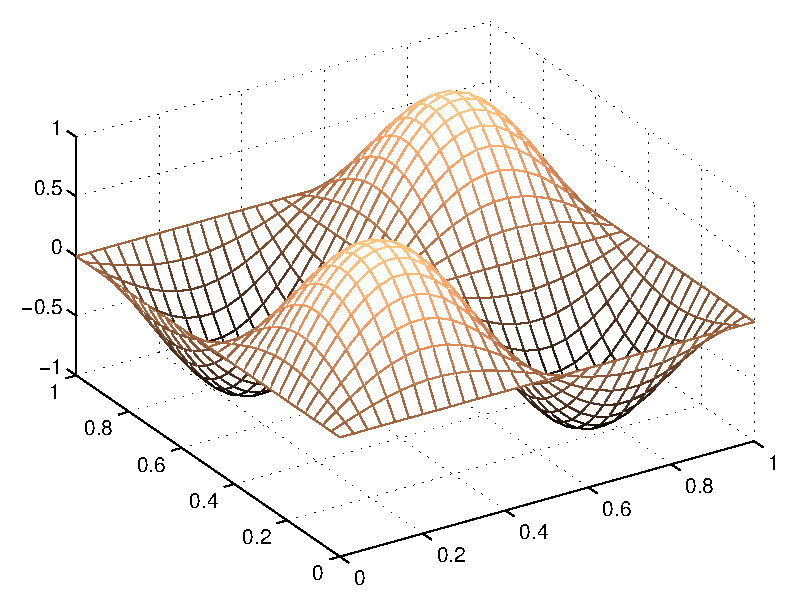
\includegraphics[width=0.4\textwidth]{figs/sine_wave_funct3}}
	}
	\subfigure[tilting slope]{
		\centering
		{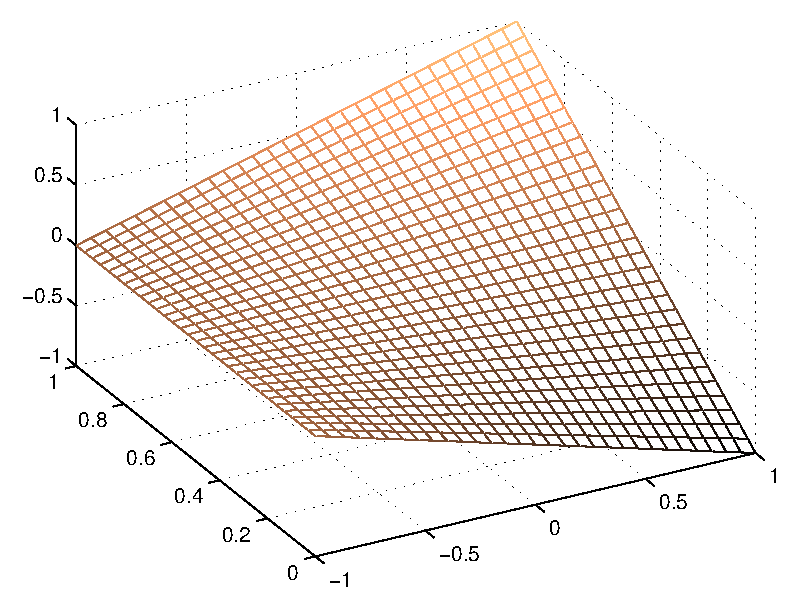
\includegraphics[width=0.4\textwidth]{figs/tilting_slope_funct3}}
	}
\caption{Two additively unfaithful functions. Relevant variables are
  zeroed out under an additive approximation because every ``slice''
  of the function integrates to zero.}
\vskip-10pt
\end{figure*}

In order to exploit additive models in variable selection, it is important to understand when the
additive approximation accurately captures all of the relevant variables.
We call this property \textit{additive faithfulness}. We first formalize the intuitive notion that a multivariate function $f$ \emph{depends on} a coordinate $x_k$.

\begin{definition}
  Let $F$ be a distribution on $C=[0,1]^p$, and $f:C \rightarrow \R$. 
We say that $f$ \textit{depends on coordinate $k$} if, for all $x_k \in [0,1]$, the set 
$\big\{ x'_k \in [0, 1] \,:\, f(x_k, \mathbf{x}_{-k}) = f(x'_k, \mathbf{x}_{-k}) 
\trm{ for almost all  $\mathbf{x}_{-k}$} \big\}$ 
has probability strictly less than one.
If $f$ is differentiable, then $f$ depends on $k$ if $\partial_{x_k} f \neq 0$ with probability greater than zero.

Suppose we have the additive approximation
\begin{equation}
\label{eqn:unconstrained_additive}
f_k^*, \mu^* \coloneqq \argmin_{f_1,\ldots, f_s, \mu} \Bigl\{ 
             \E \Bigl[\Bigl( f(X) - \sum_{k=1}^p f_k(X_k) -\mu \Bigr)^2 \Bigr]
         \,:\, \E f_k(X_k) = 0 \Bigr\}.
\end{equation}
We say that $f$ is \textit{additively faithful} under $F$ in case
$f^*_k = 0$ implies that $f$ does not depend on coordinate $k$.
\end{definition}

% We can define the support $\trm{supp}(f) \coloneqq \{ k \,:\,
% \trm{$k$ is relevant to $f$}\}$. Let $f^* = \sum_{k=1}^p$, then $f$
% is additively faith if $\trm{supp}(f) = \trm{supp}(f^*)$.

Additive faithfulness is an attractive property because it implies
that, in the population setting, the additive approximation yields
consistent variable selection.

\subsection{Additive Faithfulness of Convex Functions}

We now show that under a general class of distributions which we
characterize below, convex multivariate functions are additively
faithful.

\begin{definition}
\label{defn:boundary-point}
A density $p(\mathbf{x})$ be a density supported on $[0,1]^p$ satisfies
the \emph{boundary points condition} if, for all $j$, and for all $\mathbf{x}_{-j}$:

\begin{equation}
\frac{\partial p(\mathbf{x}_{-j} \given x_j)}{\partial x_j}  =  
\frac{\partial^2 p(\mathbf{x}_{-j} \given x_j)}{\partial x_j^2} = 0
\quad \trm{at } x_k = 0, x_k = 1
\end{equation}

\end{definition}



The boundary points condition is a weak condition. For instance, it is
satisfied when the density is flat at the boundary of support---more
precisely, when the joint density satisfies the property that
$\frac{\partial p(x_j,\mathbf{x}_{-j})}{\partial x_j} =
\frac{\partial^2 p(x_j, \mathbf{x}_{-j})}{\partial x_j^2} = 0$ at
points $x_j = 0, x_j=1$. The boundary points property is also
trivially satisfied when $p$ is a product density.

The following theorem is the main result of this section.

\begin{theorem}
\label{thm:convex_faithful}
Let $p$ be a positive density supported on $C=[0,1]^p$ that satisfies
the boundary points property. 
If $f$ is convex and twice differentiable, then $f$ is additively faithful under $p$.
\end{theorem}

% We give the full proof in Section~\ref{sec:faithful_proof} of the
% Appendix, but pause here to provide some intuition. 

We pause to give some intuition before we presenting the full proof.
Suppose that the the underlying distribution has a product density.
Then we know from Lemma~\ref{lem:general_int_reduction} that the
additive approximation zeroes out $k$ when, fixing $x_k$, every
``slice'' of $f$ integrates to zero. We prove
Theorem~\ref{thm:convex_faithful} by showing that ``slices'' of convex
functions that integrate to zero cannot be ``glued'' together while
still maintaining convexity.


\begin{proof}

Fixing $k$ and using the result of
Lemma~\ref{lem:general_int_reduction}, 
we need only show that for all $x_k$, $ \E[ f(X) - \sum_{k'}
f_{k'}(X_{k'}) \given x_k] - \E f(X) = 0 $ 
implies that $f$ does not depend on coordinate $k$, i.e., 
$\partial_{x_k} f(\mathbf{x}) = 0$ for all $\mathbf{x}$.

Let us use the shorthand notation that $r(\mathbf{x}_{-k}) = \sum_{k'
  \neq k} f_{k'}(x_{k'})$ and assume without loss of generality that
$\mu = 0$. We then assume that for all $x_k$,
\begin{equation}
 \E[ f(X) - r(X_{-k})  \given x_k] \equiv 
 \int_{\mathbf{x}_{-k}}  p(\mathbf{x}_{-k} \given x_k ) 
 \big(f(\mathbf{x}) - r(\mathbf{x}_{-k}) \big) = 0.
\end{equation}
We let $p'(\mathbf{x}_{-k} \given x_k)$ denote 
$\frac{\partial p(\mathbf{x}_{-k} \given x_k)}{\partial x_k}$ and 
$p''(\mathbf{x}_{-k} \given x_k)$ denote 
$\frac{\partial^2 p(\mathbf{x}_{-k} \given x_k)}{\partial x_k^2}$ and
likewise for $f'(x_k, \mathbf{x}_{-k})$ and $f''(x_k,
\mathbf{x}_{-k})$. We then differentiate under the integral, valid
because all functions are bounded, and obtain
\begin{gather}
\int_{\mathbf{x}_{-k}} p'(\mathbf{x}_{-k} \given x_k) 
\big( f(\mathbf{x}) - r(\mathbf{x}_{-k}) \big) + 
p(\mathbf{x}_{-k} \given x_k) f'(x_k, \mathbf{x}_{-k}) d \mathbf{x}_{-k}  = 0 
\label{eqn:integral1a} \\
\int_{\mathbf{x}_{-k}} p''(\mathbf{x}_{-k} \given x_k) 
\big( f(\mathbf{x}) - r(\mathbf{x}_{-k}) \big)  + 2 p'(\mathbf{x}_{-k} \given x_k) f'(x_k, \mathbf{x}_{-k}) +
p(\mathbf{x}_{-k} \given x_k) f''(x_k, \mathbf{x}_{-k}) d\mathbf{x}_{-k}  = 0 .
\end{gather}

By the boundary points condition, we have that $p''(\mathbf{x}_{-k}
\given x_k)$ and $p'(\mathbf{x}_{-k} \given x_k)$ are zero at $x_k =
x_k^0 \equiv 0$. The integral equations then reduce to the following:
\begin{align}
& \int_{\mathbf{x}_{-k}} p(\mathbf{x}_{-k} \given x^0_k) f'(x^0_k, \mathbf{x}_{-k}) d \mathbf{x}_{-k}= 0 \label{eqn:integral1b} \\
& \int_{\mathbf{x}_{-k}} p(\mathbf{x}_{-k} \given x^0_k) f''(x^0_k, \mathbf{x}_{-k}) d\mathbf{x}_{-k} = 0.
\end{align}
Because $f$ is convex, $f(x_k, \mathbf{x}_{-k})$ must be a convex
function of 
$x_k$ for all $\mathbf{x}_{-k}$. Therefore, for all $\mathbf{x}_{-k}$,
$f''(x^0_k, \mathbf{x}_{-k}) \geq 0$. Since $p(\mathbf{x}_{-k} \given
x^0_k) > 0$ by the assumption that $p$ is a positive density, 
we have that $\forall \mathbf{x}_{-k}, f''(x^0_k, \mathbf{x}_{-k}) = 0$ necessarily.

The Hessian of $f$ at $(x^0_k, \mathbf{x}_{-k})$ then has a zero at
the $k$-th main diagonal entry. A positive semidefinite matrix with a
zero on the $k$-th main diagonal entry must have only zeros on the
$k$-th row and column; see proposition 7.1.10 of
\citet{HJ90}.  Thus, at all $\mathbf{x}_{-k}$, the
gradient of $f'(x^0_k, \mathbf{x}_{-k})$ with respect to
$\mathbf{x}_{-k}$ must be zero.
Therefore, $f'(x_k^0, \mathbf{x}_{-k})$ must be constant for all
$\mathbf{x}_{-k}$. By equation~\ref{eqn:integral1b}, we conclude 
that $f'(x_k^0, \mathbf{x}_{-k}) = 0$ for all $\mathbf{x}_{-k}$. We
can use the same reasoning for the case where $x_k = x_k^1$ and deduce
that $f'(x^1_k, \mathbf{x}_{-k}) = 0$ for all $\mathbf{x}_{-k}$. 

Because $f(x_k, \mathbf{x}_{-k})$ as a function of $x_k$ is convex, it must be that, for all $x_k \in (0,1)$ and for all $\mathbf{x}_{-k}$,
\begin{equation}
0 = f'(x_k^0, \mathbf{x}_{-k}) \leq f'(x_k, \mathbf{x}_{-k}) \leq 
    f'(x_k^1, \mathbf{x}_{-k}) = 0
\end{equation}
Therefore $f$ does not depend on $x_k$.
% Now we apply the first-order condition of convex functions to any two points $(x_k, \mathbf{x}_{-k})$ and $(x'_k, \mathbf{x}_{-k})$ where $x_k, x'_k \in [0,1]$:

% \begin{align*}
% \forall \mathbf{x}_{-k}, f(x'_k, \mathbf{x}_{-k}) & \leq f(x_k, \mathbf{x}_{-k}) 
%   + f'(x_k, \mathbf{x}_{-k}) ( x'_k - x_k) \\ 
% f(x'_k, \mathbf{x}_{-k}) &\leq f(x_k, \mathbf{x}_{-k}) \\
% \forall \mathbf{x}_{-k}, f(x_k, \mathbf{x}_{-k}) & \leq f(x'_k, \mathbf{x}_{-k}) 
%   + f'(x'_k, \mathbf{x}_{-k}) ( x_k - x'_k) \\ 
% f(x_k, \mathbf{x}_{-k}) &\leq f(x'_k, \mathbf{x}_{-k})
% \end{align*}

% We thus have that $f(x_k, \mathbf{x}_{-k}) = f(x'_k, \mathbf{x}_{-k})$ for all $\mathbf{x}_{-k}$ and all pairs $x_k, x'_k \in (0,1)$. This proves that $f$ does not depend on $x_k$.
\end{proof}

Theorem~\ref{thm:convex_faithful} plays an important role in our
finite sample analysis, where we show that the additive
approximation is variable selection consistent (or ``sparsistent''), even when the true function is not
additive.

\begin{remark}
  We assume twice differentiability in
  Theorems~\ref{thm:convex_faithful} to simplify the proof.  We
  expect, however, that this this smoothness condition is not
  necessary---every convex function can be approximated arbitrarily
  well by a smooth convex function.
\end{remark}

\begin{remark} 
  We have not found natural conditions under which the opposite
  direction of additive faithfulness holds---conditions implying that if $f$ does not
  depend on coordinate $k$, then $f_k^*$ will be zero in the additive
  approximation.  Suppose, for example, that $f$ is only a
  function of $X_1, X_2$, and that $(X_1, X_2, X_3)$ follows a
  degenerate 3-dimensional distribution where $X_3 = f(X_1, X_2) -
  f^*(X_1) - f^*_2(X_2)$.  In this case $X_3$ exactly captures the
  additive approximation error.  The best additive
  approximation of $f$ would have a component $f^*_3(x_3) = x_3$ even
  though $f$ does not depend on $x_3$.
\end{remark}

\begin{remark}
It is possible to get a similar result for distributions with
unbounded support, by using a limit condition $\lim_{|x_k| \rightarrow
  \infty} \frac{\partial p(\mathbf{\scriptstyle x}_{-k} \given x_k)}{\partial x_k}
= 0$.  Such a limit condition is too
strong however, as it is not obeyed by the multivariate Gaussian
distribution. 
\end{remark}

The following example shows that not all convex functions are
additively faithful under multivariate Gaussian distributions.

\begin{example}
\label{examp:gaussian_counterexample}
Consider a quadratic form $f( \mathbf{x}) = \mathbf{x}^\tran H \mathbf{x} + c^\tran \mathbf{x}$ and a Gaussian distribution $X \sim N(0, \Sigma)$ where $\Sigma_{jj} = 1$ for all $j$.
As we show in the appendix, the additive approximation has the
following closed form.
\begin{enumerate}
\item If $f$ does not depend on $x_j$, then $f^*_j(x_j) = 0$.
\item If $f$ depends on $x_j$, then
\begin{equation}
f^*_j(x_j) = H_j^\tran \Sigma_j x_j^2 + c_j x_j
\end{equation}
where $H_j, \Sigma_j$ are the $j$-th rows of $H_j, \Sigma_j$, respectively. 
\end{enumerate}
Let $H = \begin{pmatrix}1 & 2 \\ 2 & 5\end{pmatrix}$ and let $\Sigma
= \begin{pmatrix}1 & -\alpha \\ -\alpha & 1\end{pmatrix}$. 
It can be checked that if if $\alpha=\frac{1}{2}$, then $f^*_1 = 0$
and additive faithfulness is violated.  Moreover, if $\alpha > \frac{1}{2}$, then $f^*_1$ is a concave function.
\end{example}

\subsection{Convex Additive Models}

Although convex functions are additively faithful, it is difficult to estimate the optimal additive functions $f^*_k$'s (as defined in equation~\ref{eqn:unconstrained_additive}) because $f^*_k$ need not be a convex function, as example~\ref{examp:gaussian_counterexample} shows. $f^*_k$ can be shown to be smooth but it is preferable to use shape-constraints whenever possible to avoid the introduction of the additional smoothing bandwidth.

Since the true regression function $f$ is convex, it is natural to ask when it is sufficient to estimate an convex additive model:
\begin{equation}
\label{eqn:convex_additive}
\{ f^*_k \}_{k=1}^p = \arg\min \Big \{ 
    \E\big( f(X) - \sum_{k=1}^p f_k(X_k) \big)^2 \,:\, f_k \in \mathcal{C}^1, \, \E f_k(X_k) = 0 \Big \}
\end{equation}
where $\mathcal{C}^1$ is the set of univariate convex functions.

The convex functions $f^*_k$'s are not additively faithful by themselves unfortunately. But, faithfulness can be restored by coupling the $f^*_k$'s with a set of concave functions:
\begin{equation}
\label{eqn:concave_postprocess}
g^*_k = \arg\min \Big\{
   \E\big( f(X) - \sum_{k' \neq k} f^*_{k'}(X_{k'}) - g_k \big)^2 
    \,:\, g_k \in \mh \mathcal{C}^1, \E g_k(X_k) = 0 
  \Big\}
\end{equation}

\begin{theorem}
\label{thm:acdc_faithful}
Suppose $p(\mathbf{x})$ is a positive density on $C=[0,1]^p$ and satisfies the boundary points condition. Suppose that $f$ is convex and twice-differentiable.

Suppose that $\partial_{x_k} f$, $\partial_{x_k} p( \mathbf{x}_{-k} \given x_k )$, and $\partial_{x_k}^2 p( \mathbf{x}_{-k} \given x_k)$ are all continuous as functions on $C$.\\

Then, $f^*_k = 0$ and $g^*_k = 0$ (as defined in equation~\ref{eqn:convex_additive} and equation~\ref{eqn:concave_postprocess}) implies that $f$ does not depend on $x_k$, i.e., $\partial_{x_k} f(\mathbf{x}) = 0$ with probability 1.
\end{theorem}

Theorem~\ref{thm:acdc_faithful} suggests a two-stage screening procedure for variable selection. We first fit a sparse \emph{convex} additive model and then, for every variable marked as irrelevant in the first stage, we allow ourself to change our mind by fitting an univariate \emph{concave} function. We refer to this procedure as AC/DC (additive convex / decoupled concave) and describe it in more details in section~\ref{sec:acdc}.

\begin{proof} (of theorem~\ref{thm:acdc_faithful}) \\
Fix $k$. Let $f^*_k, g^*_k$'s be defined as equation~\ref{eqn:convex_additive} and equation~\ref{eqn:concave_postprocess}.

By definition of $f^*_k$ and $g^*_k$, we have that:
\begin{align*}
f^*_k &= \arg\min_{f_k} \Big\{
   \E\big( f(X) - \sum_{k' \neq k} f^*_{k'}(X_{k'}) - g_k \big)^2 
    \,:\, f_k \in  \mathcal{C}^1,\, \E f_k(X_k) = 0 
  \Big\} \\
g^*_k &= \arg\min_{g_k} \Big\{
   \E\big( f(X) - \sum_{k' \neq k} f^*_{k'}(X_{k'}) - g_k \big)^2 
    \,:\, g_k \in \mh \mathcal{C}^1,\, \E g_k(X_k) = 0 
  \Big\}
\end{align*}

Therefore, $f^*_k = 0$ and $f^*_k = 0$ implies that $\E[ f(X) - \sum_{k'\neq k} f^*_{k'}(X_{k'}) \given x_k] = 0$.

Now we use corollary~\ref{cor:faithfulness_extension}. We let $\phi(\mathbf{x}_{-k}) = f(\mathbf{x}) - \sum_{k' \neq k} f^*_{k'} (x_{k'})$ and conclude that $f$ does not depend on $x_k$. 
\end{proof}


\begin{corollary} 
\label{cor:faithfulness_extension}
Suppose $p(x)$ is a positive density on $[0,1]^p$ and it satisfies the boundary points condition.

For any function $\phi(X_{-k})$ that does not depend on $X_k$:
 \begin{align*}
f^*_k(x_k) &= \arg\min_{f_k} \mathbb{E} \Big( f(X) 
           - \phi(X_{-k}) - f_k(X_k) \Big)^2 
      = \mathbb{E}\Big[ f(X) - \phi(X_{-k}) \,|\, x_k\Big] 
\end{align*}
We have that $ f^*_k = 0 \Rightarrow \partial_{x_k} f(x) = 0$.
\end{corollary}

\begin{proof}
In the proof of theorem~\ref{thm:convex_faithful}, the only property of $r(\mathbf{x}_{-k})$ we used was the fact that $\partial_{x_k} r(\mathbf{x}_{-k}) = 0$. Therefore, the proof here is identical to that of theorem~\ref{thm:convex_faithful} except we let $\phi(\mathbf{x}_{-k})= r(\mathbf{x}_{-k}).$
\end{proof}


\begin{proposition}
\label{prop:shape_approx_univariate}
Let $C \subset \R^p$ be a compact set and let $h : C \rightarrow \R$. Let $p(x)$ be a positive density on $C$ and suppose $\E h(X) = 0$. Suppose that $\partial_{x_k} h(x)$, $\partial_{x_k} p( x \given x_k)$, and $\partial^2_{x_k} p( x \given x_k )$ are all continuous as functions on $C$. Suppose that $\partial^2_{x_k} h(x) \geq 0$.


Let 
\begin{align*}
f^*_k(x_k) &= \arg\min_{f_k} \Big\{
   \E \Big( h(X) - f_k(X_k) \Big)^2 \,:\, f_k \in \mathcal{C}^1,\, \E f_k = 0 \Big\} \\
g^*_k(x_k) &= \arg\min_{g_k} \Big \{
   \E \Big( h(X) - g_k(X_k) \Big)^2 \,:\, g_k \in \mh \mathcal{C}^1 ,\, \E g_k = 0 \Big\}
\end{align*}
be the best convex and concave univariate approximation respectively.\\

Then, $f^*_k = 0$ and $g^*_k = 0$ iff $h^*_k(x_k) \equiv \E[ h(X) \given x_k ] = 0$.
\end{proposition}

\begin{proof}


First, we will establish that $h^*_k(x_k)$ is twice differentiable and that $\partial^2_{x_k} h^*_k(x_k)$ is lower bounded. 

\begin{align*}
h^*_k(x_k) &= \E[ h(X) \given x_k] \\
  &= \int_{x_{-k}} h(x) p(\mathbf{x}_{-k} \given x_k) d \mathbf{x}_{-k}\\
\partial^2_{x_k} h^*_k(x_k) 
  &= \int_{\mathbf{x}_{-k}} h''(\mathbf{x}) p(\mathbf{x}_{-k} \given x_k) +
  2 h'(x) p'(\mathbf{x}_{-k} \given x_k) + h(x) p''(\mathbf{x}_{-k} \given x_k) 
  d\mathbf{x}_{-k} 
\end{align*}

The first term $h''(x) p(\mathbf{x}_{-k} \given x_k)$ is strictly positive. By assumption, the remaining terms are continuous and hence bounded on a compact set. $\partial^2_{x_k} h^*_k(x_k)$ is therefore lower bounded. Before proceeding, we also note that because $\E h(X) = 0$, it must be that $\E h^*_k(X_k) = 0$.

Now suppose $f^*_k = 0$ and $g^*_k = 0$. Let $\sigma_k^2$ denote $\E X_k^2$. Then 
\begin{equation}
\arg\min_{c \in \mathbb{R}} \mathbb{E}\Big( h(X) - c (X_k^2-\sigma_k^2) \Big)^2 = 0
\end{equation}
Since optimal $c^* = \frac{\mathbb{E} [ h(X) (X_k^2-\sigma_k^2) ]}{\mathbb{E}[ X_k^2 ]}$, 
we know $\mathbb{E} [ h(X) X_k^2 ] = 
\mathbb{E} \Big[ \mathbb{E}[ h(X) \,|\, X_k] X_k^2 \Big] = 0$.\\

Because $\partial^2_{x_k} h^*_k(x_k)$ is lower bounded, for large enough $\alpha$, $h^*_k(x_k) + \alpha (x_k^2 - \sigma_k^2)$ has a non-negative second derivative and thus is convex. Then
\begin{equation}
\arg\min_{c \in \mathbb{R}} \mathbb{E}\Big( h(X) 
       - c (h^*_k(X_k) + \alpha (X_k^2 - \sigma_k^2)) \Big)^2 = 0
\end{equation}
Again, $c^* = \frac{\mathbb{E}[g(X)\big( 
            h^*_k(X_k) + \alpha (X_k^2 - \sigma_k^2) \big)]}{\mathbb{E}
        \big( h^*_k(X_k) + \alpha (X_k^2 - \sigma_k^2) \big)^2} = 0$, so
\begin{align*}
\mathbb{E}[ h(X) \big( h^*_k(X_k) + \alpha X_k^2 \big) ] &= 
\mathbb{E}[ h(X) h^*_k(X_k) ] \\
& = \mathbb{E}\Big[ \mathbb{E}[h(X) | X_k]  h^*_k(X_k) \Big] \\
& = \mathbb{E} h^*_k(X_k)^2 = 0
\end{align*}
Therefore, $h^*_k(x_k) = 0$.

\end{proof}


% \begin{remark}
% Without restrictions on the distribution, a convex
%   function may not be additively faithful. Intuitively, an arbitrarily shaped
%   density $p$
%   may ``undo'' the convexity of $f$ so that the product
%   $p(\mathbf{x}) \, f(\mathbf{x})$ resembles an egg carton or a
%   tilting slope.  With appropriate conditions on the density $p$,
%   however, it is possible to relax the independence assumption.  We leave this to
%   future work.
% \end{remark}


% DO NOT CHANGE; RefTex variables -minx
 
%%% Local Variables: ***
%%% mode:latex ***
%%% TeX-master: "paper.tex" ***
%%% End: ***

